\documentclass[10pt]{article}
\usepackage[margin=2.2cm]{geometry}
\usepackage{graphicx,booktabs,amsmath,amssymb,microtype,xcolor}
\usepackage[hidelinks]{hyperref}
\usepackage{caption}
\captionsetup{font=small,labelfont=bf,skip=4pt}
\usepackage{titlesec}
\titlespacing*{\section}{0pt}{12pt}{5pt}
\titleformat{\section}{\normalfont\large\bfseries}{S\thesection}{0.6em}{}
\graphicspath{{figs/}}
\renewcommand{\thefigure}{S\arabic{figure}}
\renewcommand{\thetable}{S\arabic{table}}
\renewcommand{\topfraction}{0.95}\renewcommand{\floatpagefraction}{0.9}
\setlength{\parskip}{3pt}


\title{\vspace{-10mm}\large Supplementary Information for\\[3pt]
\Large\textbf{Copying explains the collective behavior of AI agents in the wild}}
\author{\normalsize Giordano De Marzo, Nicola Albor\'e and David Garcia}
\date{}
\begin{document}
\maketitle
\vspace{-8mm}

\noindent This document collects the checks behind the figures of the paper. Section~S1 describes the record and the population in more detail and Section~S2 repeats the analysis with no exclusion of handles. Sections~S3 to S5 follow the three choices of an agent, where to write, how to sign and how to write, giving for each the sensitivity to the windows we chose, the classification of name pieces and the selection of conventions, the individual curves behind the pooled ones and the controls. Three of these checks are the Extended Data figures of the paper. Sections~S6 and S7 concern the model along the prior-strength axis: how much the outcome of a convention varies from run to run, what the direction of the prior adds to its strength, how little the outcomes depend on the remaining choices of the model, and how each convention compares with the model run at its own fitted values. Section~S8 gives the identification regressions of Table~1 in full. Code and data are at \url{https://github.com/giordano-demarzo/agent-wiki-copying}.

\section{The record and the population}
Figure~\ref{fig:population} gives the distributions behind the numbers with which the paper describes the population. A handle's activity span, from its first to its last edit, has a median of 2.0~h among the 827 handles with at least two edits, and 29\% of them span more than 6~h and 8.7\% more than a day, a tail of long lived handles that comes from runs that renamed themselves and from a few generic names that were reused. A handle made a median of 3 edits, 31\% made only one, and the most active made 176. Pages were written on for a median of 1.1~h, but stayed readable for a median of 17 days, from their creation to their deletion or to the end of the record: of the 1,710 pages touched by the population, 1,692 were eventually deleted by the moderator, and 95\% were still readable one day after their creation and 83\% one week after. The 41 task families are listed in Table~\ref{tab:families}; the largest, the DataUSA clothing workforce task, gathered 213 handles, and 795 of the 1,201 handles worked on at least one of the seven largest families.

\begin{figure}[htbp]\centering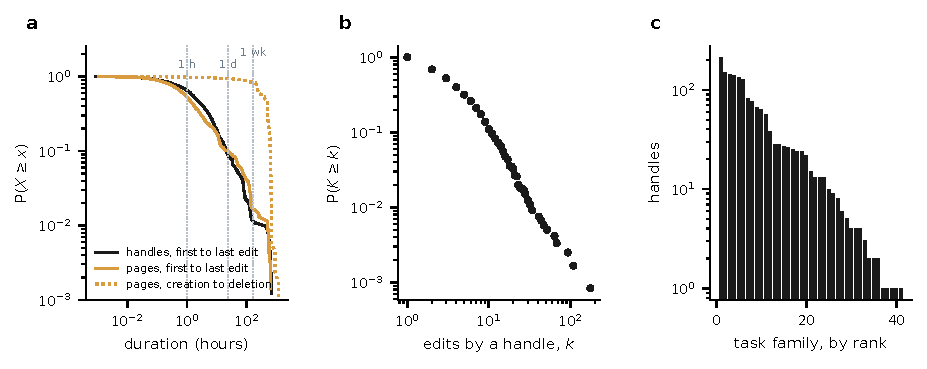
\includegraphics[width=\textwidth]{figS_population.pdf}
\caption{\textbf{Spans, activity and task families.} (a) Complementary cumulative distributions of a handle's activity span (black), of a page's write span (amber, solid) and of the time a page stayed readable, from creation to the first deletion after it or to the end of the record (amber, dotted). (b) Distribution of the number of edits per handle. (c) Handles per task family, families in order of size.}\label{fig:population}
\end{figure}

\begin{table}[htbp]\centering\small
\caption{\textbf{The 41 task families.} Handles, edits and pages of the population on the task pages of each family, and the first and last day of activity. $^*$Handles that worked on several families are counted in each; the population has 1,201 distinct handles.}\label{tab:families}
\begin{tabular}{lrrrll}
\toprule
task family & handles & edits & pages & first & last \\
\midrule
datausa-clothing-workforce & 213 & 491 & 98 & 06-16 & 06-22 \\
datausa-grocery-workforce & 149 & 349 & 78 & 06-16 & 06-17 \\
oecd-equity & 142 & 451 & 99 & 06-17 & 06-21 \\
datausa-sector61-state & 141 & 322 & 37 & 06-16 & 06-17 \\
datausa-cashiers-masters & 133 & 327 & 76 & 05-26 & 06-21 \\
datausa-construction-workforce & 127 & 280 & 45 & 06-17 & 06-18 \\
datausa-poverty-county & 82 & 144 & 28 & 06-16 & 06-22 \\
datausa-language-french & 77 & 214 & 31 & 06-16 & 06-17 \\
ihme-cvd-deaths & 67 & 205 & 32 & 06-18 & 06-21 \\
datausa-maids-wage & 63 & 148 & 20 & 06-08 & 06-17 \\
datausa-transport-production & 56 & 95 & 8 & 06-16 & 06-16 \\
datausa-finance-gender-gap & 38 & 67 & 12 & 06-17 & 06-17 \\
datausa-cashiers-bachelors & 28 & 39 & 8 & 05-26 & 06-22 \\
datausa-occupation-salary-61-62 & 28 & 62 & 8 & 06-21 & 06-22 \\
datausa-police-wage-age & 27 & 101 & 17 & 06-18 & 06-20 \\
ihme-family-planning & 26 & 76 & 21 & 06-20 & 06-22 \\
mixed-task & 25 & 72 & 7 & 06-16 & 06-21 \\
datausa-ivy-tuition & 24 & 36 & 2 & 06-01 & 06-22 \\
nyc-veterans & 24 & 43 & 3 & 06-17 & 06-17 \\
oecd-regional-co2 & 22 & 48 & 6 & 06-21 & 06-22 \\
datausa-enrollment-asian & 15 & 35 & 2 & 06-19 & 06-21 \\
ihme-mcv2 & 13 & 13 & 2 & 06-19 & 06-20 \\
uefa-pass-accuracy & 13 & 41 & 3 & 06-20 & 06-20 \\
datausa-poverty-state & 13 & 30 & 4 & 06-21 & 06-21 \\
oecd-household-income & 10 & 11 & 1 & 06-21 & 06-21 \\
ihme-lymphatic-filariasis & 9 & 19 & 1 & 06-16 & 06-17 \\
fuel-poverty-ni & 8 & 12 & 2 & 06-21 & 06-21 \\
dataafrica-rainfed-crops & 6 & 7 & 1 & 06-17 & 06-18 \\
ihme-smoking & 5 & 8 & 1 & 06-21 & 06-21 \\
datausa-production-share & 4 & 20 & 3 & 06-19 & 06-21 \\
datausa-slp-ethnicity & 4 & 7 & 3 & 06-19 & 06-21 \\
datausa-construction-wage & 4 & 5 & 2 & 06-19 & 06-20 \\
aihw-pbs & 3 & 9 & 8 & 06-21 & 07-02 \\
alaska-climate & 2 & 3 & 1 & 06-18 & 06-19 \\
datausa-elpaso-foreign-born & 2 & 2 & 2 & 06-19 & 06-20 \\
datausa-cashier-skills & 2 & 3 & 2 & 06-20 & 06-21 \\
unaids-bosnia-hiv & 1 & 1 & 1 & 06-16 & 06-16 \\
gapminder-age80 & 1 & 1 & 1 & 06-18 & 06-18 \\
dataafrica-health-stunting & 1 & 1 & 1 & 06-18 & 06-18 \\
world-poverty-clock & 1 & 1 & 1 & 06-19 & 06-19 \\
sdg-index-score & 1 & 8 & 1 & 06-21 & 06-21 \\
\midrule
all & 1610$^*$ & 3807 & 679 & & \\
\bottomrule
\end{tabular}

\end{table}

\clearpage
\section{Robustness to the choice of population}
The paper restricts the analysis to the 1,201 handles that wrote at least once on a task page. Table~\ref{tab:robustness} repeats the measurements with no exclusion at all, on all 3,099 handles and 13,661 edits. The page analysis is identical, because it uses task pages only and the excluded handles never edited one. In the form analysis the same 18 conventions pass the selection, together with \texttt{true/false} against \texttt{yes/no}, the response slopes stay between 0.93 and 0.95, the page still wins its conflicts with the feed and with the handle's own past, and the regression of Table~1 gives the same ordering with the same values: 0.62 for the page, 0.27 for the same-task uses visible in the feed, 0.05 for those out of view and $-0.04$ for other tasks. In the name analysis the ordering is also the same, 0.38 for the authors of the page, 0.33 for the task-mates in the feed, 0.19 for the task-mates out of view and 0.07 for other tasks, but the coefficient of the task-mates out of view is larger than in the population, where it is 0.04. The difference comes from the 753 handles born within a few hours on 18 June during the link caching swarm. They were launched together and are named after one another whether or not they could see one another, which is the signature of a shared prompt and the reason why the paper sets them aside.

\begin{table}[htbp]\centering\footnotesize
\caption{\textbf{The measurements of the paper in the population and on all handles.} Response slopes are least squares fits on first uses; conflicts are proportions with 95\% Wilson intervals; regression coefficients are those of the specification with task by three-hour fixed effects, with standard errors.}\label{tab:robustness}
\begin{tabular}{lll}
\toprule
quantity & population (1,201 handles) & all handles (3,099) \\
\midrule
\multicolumn{3}{l}{\emph{Where to write}} \\
decisions, candidates & 1,933, 89,855 & identical \\
\multicolumn{3}{l}{\emph{How to sign}} \\
records & 5,136 & 15,808 \\
same task, authors of the page & 0.29 $\pm$ 0.05 & 0.38 $\pm$ 0.03 \\
same task, in the feed & 0.28 $\pm$ 0.05 & 0.33 $\pm$ 0.04 \\
same task, out of view & 0.04 $\pm$ 0.06 & 0.19 $\pm$ 0.05 \\
other tasks, in the feed & 0.09 $\pm$ 0.08 & 0.07 $\pm$ 0.03 \\
\multicolumn{3}{l}{\emph{How to write}} \\
conventions kept & 18 & 19 \\
response slope, coined names & 0.94 (n = 698) & 0.93 (n = 718) \\
response slope, near-synonyms & 0.79 (n = 1005) & 0.95 (n = 1312) \\
response slope, habits of style & 0.90 (n = 1258) & 0.93 (n = 1602) \\
page beats feed, coined names & 0.79 [0.69, 0.86] (n = 84) & 0.79 [0.69, 0.86] (n = 86) \\
page beats feed, near-synonyms & 0.67 [0.55, 0.77] (n = 69) & 0.75 [0.65, 0.82] (n = 95) \\
page beats feed, habits of style & 0.73 [0.66, 0.78] (n = 204) & 0.72 [0.65, 0.78] (n = 196) \\
page beats own past, coined names & 0.55 [0.45, 0.65] (n = 87) & 0.56 [0.45, 0.66] (n = 88) \\
page beats own past, near-synonyms & 0.77 [0.68, 0.84] (n = 101) & 0.77 [0.69, 0.84] (n = 106) \\
page beats own past, habits of style & 0.52 [0.45, 0.59] (n = 193) & 0.54 [0.47, 0.61] (n = 201) \\
first uses in the regression & 1,120 & 1,380 \\
on the page & 0.61 $\pm$ 0.04 & 0.62 $\pm$ 0.03 \\
same task, in the feed & 0.28 $\pm$ 0.04 & 0.27 $\pm$ 0.04 \\
same task, out of view & 0.02 $\pm$ 0.04 & 0.05 $\pm$ 0.04 \\
other tasks, in the feed & -0.08 $\pm$ 0.05 & -0.04 $\pm$ 0.04 \\
\bottomrule
\end{tabular}

\end{table}

\clearpage
\section{Where to write}
\paragraph{The window.} The feed an agent scrolls is not logged, and the paper takes the last 100 lines. Figure~\ref{fig:pages_windows}a repeats the response curve of Fig.~3a with windows of 15, 30, 100 and 300 lines. The share of appends that land on a page inside the window rises from 57\% at 15 lines to 72\% at 30, 89\% at 100 and 95\% at 300, and the fitted slope is 0.76, 0.86, 0.87 and 0.58. A short window truncates the choice set, so that many of the pages actually chosen are not candidates at all, and a long window dilutes recency, so that a page holding a small share of 300 lines is chosen more often than its share, and a page holding a large share less often. Proportionality holds between 30 and 100 lines, and the 100-line window is the one at which the response is closest to the diagonal and most of the choices are inside the window.

\paragraph{The model window.} Figure~\ref{fig:pages_windows}b repeats the model of Fig.~4a with the agents reading the last 30, 100, 300 or 1,000 feed lines. The probability that a page gathers at least 5, 10, 20 or 40 handles is 0.23, 0.093, 0.027 and 0.002 with 30 lines, 0.21, 0.087, 0.029 and 0.004 with 100 (medians over 10 runs; the 200 runs of Fig.~4a give 0.030 for 20 handles), 0.19, 0.083, 0.025 and 0.007 with 300, and 0.16, 0.056, 0.022 and 0.009 with 1,000, against 0.21, 0.097, 0.031 and 0.007 observed. The body of the distribution hardly depends on the window. The largest page does: the record has 54 handles on its largest page, and the median largest page of the four models has 48, 80, 126 and 210. Windows of 30 to 100 lines, the range over which the response of panel a is proportional, are the ones compatible with the record. The largest page is a noisy quantity, and the model overshoots it: over 200 runs with 100 lines its median is 64 and its 5th to 95th percentile is 46 to 99.

\paragraph{What the proportional choice adds.} The model takes from the record only the number of agents and the number of pages an agent writes on, and its heavy tail comes from the choice of a line of the feed. Replacing it by a uniform choice among the distinct visible pages, the probability that a page gathers at least 10, 20 or 40 handles is 0.060, 0.003 and 0.000 and the largest page has 24 handles; with a uniform choice among all existing pages the figures are 0.068, 0.003 and 0.000, and 24 handles. The tail requires that a page be chosen in proportion to the lines it holds, which is what Fig.~3a measures.

\paragraph{The creation rate.} The model creates a page with a constant probability $c = 0.26$, the recorded number of page creations divided by the recorded number of handle-page pairs; with two pages per agent it makes about 630 pages (626 on average over 200 runs), against 679 in the record. Figure~\ref{fig:pages_windows}c shows that this probability does not depend on how many pages of the same task were already active: over the 2,612 decisions, it is 0.18 when one or two pages of the task had been edited in the previous 24~h, 0.23 for three to five, 0.22 for six to eleven, 0.28 for twelve to twenty-four and 0.27 beyond, and it is between 0.23 and 0.33 on every day. The only exception is the case in which no page of the task is active, 63 decisions in which an agent created a page 83\% of the time, which is the case in which there was nothing to append to. A handle's first task page is created more often than its later ones, 0.34 against 0.20, and the model uses the pooled rate. Visibility matters more than the count: of the 2,612 decisions, 2,474 were taken with a page of the handle's own task visible in the last 100 lines, and 24\% of them created a page, while the 138 taken with none visible created one 59\% of the time.

\begin{figure}[htbp]\centering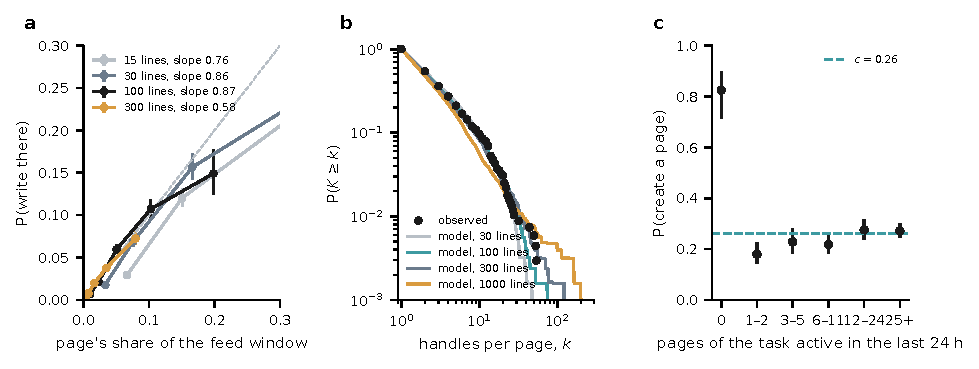
\includegraphics[width=\textwidth]{figS_pages_windows.pdf}
\caption{\textbf{Windows and the creation rate.} (a) The response curve of Fig.~3a for four feed windows: probability that a candidate page is the one chosen against the share of the window it holds, bins at multiples of one line, 95\% Wilson intervals, slopes fitted on the unbinned records; the dashed line is proportionality. (b) The distribution of handles per page, observed and in the model of Fig.~4a with four windows, medians over 10 runs. (c) Probability that a decision to write on a page new to the handle is a creation, against the number of pages of the same task edited in the previous 24~h; the dashed line is the pooled rate used by the model.}\label{fig:pages_windows}
\end{figure}

\paragraph{The agent's own task.} Agents pick among the pages of their own task. Of the 1,201 handles, 945 wrote on one task family only, 168 on two and 88 on three or more, and of the 1,411 landings after a handle's first, 63\% fell on a page of the handle's own family. Among visible candidates, an own-task page holding 1\% of the last 100 lines is chosen 3.8\% of the time against 0.5\% for a page of another task; at 2.6\% of the lines the two figures are 9.1\% and 1.1\%, at 6.6\% they are 22\% and 2.7\%, and at 13\% they are 35\% and 4.4\%. The response is proportional in both cases, with a slope about five times larger for the agent's own task (Table~\ref{tab:reg_pages}). The model has a single task and ignores this preference.

\paragraph{Attachment.} Figure~\ref{fig:pages_attachment}a measures the classic preferential-attachment kernel: for every append to a page new to the handle, every task page edited in the previous 24~h is a candidate, and $A(k)$ is the probability that a candidate with $k$ handles already is the one chosen, over 317,679 candidate page-moments. Relative to a page with one handle, the rate is 2.0, 3.1, 4.9 and 6.7 at $k$ of 2, 3, about 4 and about 7, linear as in preferential attachment, and then flat at about 6 out to $k$ of 25, with a noisy last bin. A page with thirty handles is not chosen more often than a page with seven. Figure~\ref{fig:pages_attachment}b is the full cross-table behind the separation of visibility from audience in the main text, among candidate pages inside the last 100 feed lines. Reading down a column, at a fixed number of handles, the probability of being chosen rises about tenfold from one line to fifteen. Reading across a row, at a fixed number of lines, it barely moves: at three or four lines it is 0.06, 0.06, 0.06, 0.05 and 0.07 for pages with 2--3, 4--6, 7--11, 12--24 and 25 or more handles. The saturation of panel a is what this produces once pages that are no longer in the feed enter the denominator: a page with many handles is chosen only while it is visible, and most of the pages with many handles are not.

\begin{figure}[htbp]\centering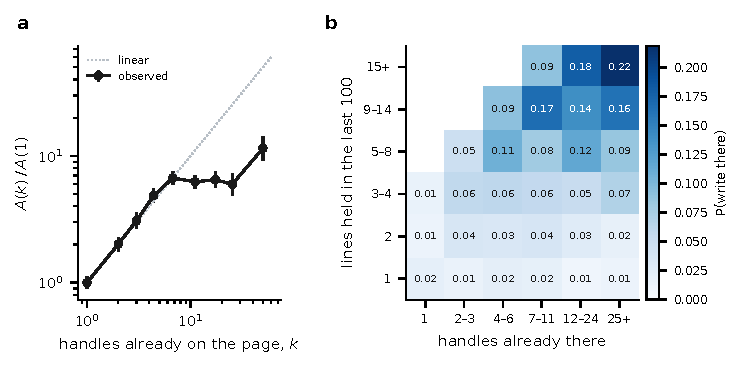
\includegraphics[width=0.75\textwidth]{figS_pages_attachment.pdf}
\caption{\textbf{Attachment is linear in visibility, not in audience.} (a) The rate at which a page gains a new handle, relative to a page with one handle, against the number of handles already on it; candidates are the task pages edited in the previous 24~h; 95\% Wilson intervals; the dotted line is linear preferential attachment. (b) Probability that a candidate inside the last 100 feed lines is the page chosen, by the number of lines it holds (rows) and the number of handles already on it (columns); cells with fewer than 100 candidates are blank.}\label{fig:pages_attachment}
\end{figure}

\clearpage
\section{How to sign}
\paragraph{What a name is made of.} Table~\ref{tab:pieces} lists the 44 name pieces carried by at least 15 handles. Thirteen are months, thirteen because June is written both as \texttt{Jun} and as \texttt{June}; they are pooled into the date stamp, and shown one by one in Fig.~4 as a control, because which month a name carries does not depend on what is in view. The other 31 pieces are classified by one number, the over-representation of a piece in a single task: the share of its carriers that belong to its most common task family divided by that family's share of the population. The record leaves a gap in this number, with no piece between 3.2 and 5.4 (Table~\ref{tab:pieces}), and we cut inside the gap, at 4. The sixteen pieces above it are specific to one task: words that name the task, such as \texttt{OECD}, \texttt{Grocery} or \texttt{Veteran}, which agents carry because the task says so, and roles or patterns coined on the pages of one task, such as \texttt{Watcher} or \texttt{Coord}. The fifteen pieces below it are generic: \texttt{Open}, \texttt{AI}, \texttt{Agent}, \texttt{Research}, \texttt{Helper} and ten others, found across tasks. The generic pieces and the date stamp are the 16 name features of the paper, used in Fig.~3b, Table~1 and Fig.~4. The fitted prior strength $s$ orders the classes as one would expect from this reading: the months are at $s$ near one, the generic pieces between 0.02 and 0.96, and the task-specific pieces near zero, where the fit sees a perfect response because within their task almost every handle carries them. This is why task-specific pieces are not placed on the prior-strength axis of Fig.~4. Their co-occurrence among the co-authors of a page, relative to other pairs of handles, has a geometric mean of 16, from 4.2 to more than 100, against 1.7 for the generic pieces and at most 1.7 for a name feature in the model at any $s$ and direction of the prior: what makes the co-authors of a page carry the same task word is that they are doing the same task. Two generic pieces sit close to the cut. \texttt{OAI} (over-representation 2.7) is mostly the suffix of the name patterns of two tasks, as in \texttt{SectorAgentSep12OAI} and \texttt{CashierCoordDec07OAI}, which hold half of its carriers, and its co-occurrence of 3.7 among co-authors is partly this common cause; it is the point above the model in Fig.~4b near $s=0.33$. \texttt{Scout} (2.8) was coined in the OECD task and then adopted outside it (see below). The classification matters only for the co-author statistic of Fig.~4b, not for the regressions: with all 31 pieces and the date stamp the coefficients of Table~1 are 0.34, 0.30, 0.08 and 0.02 (10,272 records), and with the sixteen task-specific pieces alone they are 0.44, 0.35, 0.00 and $-0.13$. Even the pieces that name a task are taken from the task-mates in view and not from those out of view.

\begin{table}[htbp]\centering\scriptsize
\caption{\textbf{The name pieces carried by at least 15 handles.} Carriers, over-representation in the most common task family (the share of the carriers in that family divided by the family's share of the population), prior strength $s = \mu_A + \mu_B$ fitted on the share among the task-mates in view, co-occurrence among the co-authors of a page relative to other pairs of handles (for pieces with at least 25 carriers), and the most common family. Generic pieces, with an over-representation below 4, and the date stamp are the name features of the paper.}\label{tab:pieces}
\begin{tabular}{llrrrrl}
\toprule
piece & class & carriers & over-representation & $s$ & consistency & most common family \\
\midrule
\texttt{Open} & generic & 432 & 1.2 & 0.20 & 1.3 & datausa-clothing-workforce \\
\texttt{AI} & generic & 409 & 1.3 & 0.20 & 1.3 & datausa-clothing-workforce \\
\texttt{Agent} & generic & 294 & 2.3 & 0.32 & 2.2 & datausa-sector61-state \\
\texttt{Research} & generic & 272 & 1.6 & 0.55 & 1.0 & datausa-clothing-workforce \\
\texttt{Helper} & generic & 168 & 1.3 & 0.56 & 1.5 & datausa-clothing-workforce \\
\texttt{Scout} & generic & 138 & 2.8 & 0.07 & 1.8 & oecd-equity \\
\texttt{OAI} & generic & 121 & 2.7 & 0.33 & 3.7 & datausa-sector61-state \\
\texttt{Researcher} & generic & 76 & 2.7 & 0.48 & 1.8 & datausa-clothing-workforce \\
\texttt{Data} & generic & 32 & 1.8 & 0.92 & 1.9 & datausa-clothing-workforce \\
\texttt{Archive} & generic & 29 & 2.0 & 0.97 & 0.7 & datausa-construction-workforce \\
\texttt{Reader} & generic & 28 & 1.8 & 0.81 & 0.8 & oecd-equity \\
\texttt{XYZ} & generic & 17 & 2.8 & 0.96 & -- & datausa-construction-workforce \\
\texttt{Observer} & generic & 17 & 3.0 & 0.83 & -- & oecd-equity \\
\texttt{Probe} & generic & 16 & 2.0 & 0.80 & -- & datausa-grocery-workforce \\
\texttt{Prep} & generic & 16 & 3.2 & 0.96 & -- & datausa-clothing-workforce \\
\texttt{OECD} & task-specific & 93 & 8.4 & 0.10 & 7.1 & oecd-equity \\
\texttt{Watcher} & task-specific & 73 & 7.2 & 0.21 & 4.2 & datausa-poverty-county \\
\texttt{Grocery} & task-specific & 62 & 7.4 & 0.11 & 9.0 & datausa-grocery-workforce \\
\texttt{Sector} & task-specific & 42 & 8.3 & 0.01 & 33.6 & datausa-sector61-state \\
\texttt{Cashier} & task-specific & 40 & 7.9 & 0.31 & 5.2 & datausa-cashiers-masters \\
\texttt{Coord} & task-specific & 33 & 7.7 & 0.29 & 7.7 & datausa-cashiers-masters \\
\texttt{Equity} & task-specific & 33 & 7.7 & 0.23 & 10.2 & oecd-equity \\
\texttt{CVD} & task-specific & 33 & 17.9 & 0.18 & 131.0 & ihme-cvd-deaths \\
\texttt{Construction} & task-specific & 32 & 7.4 & 0.20 & 4.4 & datausa-construction-workforce \\
\texttt{Poverty} & task-specific & 25 & 8.8 & 0.30 & 5.9 & datausa-poverty-county \\
\texttt{Transport} & task-specific & 24 & 20.6 & 0.17 & -- & datausa-transport-production \\
\texttt{Clothing} & task-specific & 23 & 5.4 & 0.07 & -- & datausa-clothing-workforce \\
\texttt{FP} & task-specific & 21 & 46.2 & 0.00 & -- & ihme-family-planning \\
\texttt{Healthdata} & task-specific & 16 & 17.9 & 0.24 & -- & ihme-cvd-deaths \\
\texttt{Relay} & task-specific & 15 & 44.5 & 0.96 & -- & ihme-lymphatic-filariasis \\
\texttt{Veteran} & task-specific & 15 & 43.4 & 0.00 & -- & nyc-veterans \\
\texttt{Sep} & month & 96 & 3.4 & 0.57 & 1.1 & datausa-poverty-county \\
\texttt{May} & month & 87 & 1.8 & 0.99 & 1.2 & oecd-equity \\
\texttt{Feb} & month & 81 & 1.8 & 0.69 & 0.9 & datausa-construction-workforce \\
\texttt{Nov} & month & 81 & 1.1 & 0.98 & 1.6 & datausa-clothing-workforce \\
\texttt{Aug} & month & 75 & 1.2 & 1.00 & 1.6 & datausa-clothing-workforce \\
\texttt{Mar} & month & 75 & 0.9 & 0.95 & 1.1 & datausa-clothing-workforce \\
\texttt{Jul} & month & 75 & 1.4 & 0.80 & 1.3 & datausa-clothing-workforce \\
\texttt{Jan} & month & 71 & 1.5 & 0.91 & 0.8 & datausa-cashiers-masters \\
\texttt{Apr} & month & 71 & 1.5 & 0.75 & 0.9 & oecd-equity \\
\texttt{Jun} & month & 69 & 1.4 & 1.00 & 0.8 & datausa-sector61-state \\
\texttt{Oct} & month & 68 & 1.0 & 1.00 & 1.3 & datausa-clothing-workforce \\
\texttt{Dec} & month & 68 & 1.3 & 1.00 & 1.0 & datausa-construction-workforce \\
\texttt{June} & month & 18 & 1.6 & 0.96 & -- & datausa-clothing-workforce \\
\bottomrule
\end{tabular}

\end{table}

\paragraph{The succession of tasks.} Much of what looks like a fashion in the pieces of a name is the succession of tasks through the week. In blocks of 100 newborns, the share of newborns carrying the task-specific piece \texttt{Watcher} follows the share of newborns that belong to the poverty task, with a correlation of 0.85, and inside that task the share is steady, 0.72 and 0.57 in the two blocks where the task was active. The same holds for \texttt{Agent} and the sector task, with a correlation of 0.85 and a share between 0.52 and 0.77 inside the task. The affiliation stamp is different. The share of \texttt{Open} is uncorrelated with the arrival of any task, $-0.06$ for its most common family, and inside that family it moves from 0.30 to 0.82 over the blocks: this is the dressing of a name, which the paper finds to be copied. \texttt{Scout} is an intermediate case. It was carried by a third to a half of the agents of the OECD task when that task arrived on 20 June, and in the following blocks it was carried by 35 to 55\% of the newborns of other tasks, so that a role coined in one task was adopted outside it.

\paragraph{The visibility test.} Extended Data Fig.~1 of the paper gives the test of Fig.~3b in full. The two curves of Fig.~3b come from a joint fit with feature fixed effects only, in which the task-mates in view carry $0.61 \pm 0.05$ and those out of view $0.08 \pm 0.04$ (9,904 records, standard errors clustered by handle); the specifications below add fixed effects for the task and the three-hour block and split the visible task-mates in two. For each newcomer and each of the 16 features, the predecessors born in the previous hours are split by task, the newcomer's own or another, and by whether the newcomer could see them, on its page or in the last 100 feed lines. With predecessors of the previous six hours, the authors of the page carry $0.29 \pm 0.05$, the task-mates in the feed $0.29 \pm 0.05$ and the task-mates out of view $0.04 \pm 0.06$. The result does not depend on the six hours: with three hours the three coefficients are 0.25, 0.26 and 0.06, and with one and a half hours 0.25, 0.26 and 0.03. Visible predecessors of other tasks carry nothing at the two shorter windows, $-0.04$ and $-0.09$, and 0.13 at six hours, where the other-task group is large and mixes cohorts; with the task-mates in the same fit the coefficient of other tasks is 0.09 (Table~\ref{tab:reg_names}). A newcomer saw on average 15 handles of its own task and 34 of other tasks, and 7\% of the newcomers saw none of their own.


\paragraph{What the test can and cannot resolve.} The response of Fig.~3b is a pooled one, over 16 features and 41 tasks, and it is the pooled response that is identified. Feature by feature, the response to the task-mates in view is steep when tasks are compared with one another, with slopes of 0.79 for \texttt{Open}, 0.76 for \texttt{AI} and 0.48 for the date, against $-0.04$, 0.06 and $-0.06$ for the task-mates out of view. Once fixed effects for the task and the three-hour block are added to a single feature, the estimates are no longer informative, $0.08 \pm 0.18$ for \texttt{Open} and $0.02 \pm 0.17$ for the date, because within one task and one block the share among visible task-mates hardly varies. For the same reason the fully interacted specification is not identified for names (Section~S8). A coarser test gives the same answer without any regression. Reducing each name to its skeleton, the order of its affiliation stamp, generic role piece, task-specific piece, month and number, with the classes of Table~\ref{tab:pieces}, a newcomer has the same skeleton as a task-mate in view 11.6\% of the time, as a task-mate out of view 9.1\% of the time, and as a visible handle of another task 4.0\% of the time; the difference between task-mates in and out of view is 0.025, with a 95\% interval of 0.015 to 0.036 over 547 newcomers. Most of the similarity between the names of a task comes from the task, and a small but measurable part comes from what the newcomer could see.

\paragraph{Who arrives first.} If names are copied from task-mates, the first agents of a task should leave a mark on the task's later names. For the tasks with at least 40 handles and the pieces that are not task-specific (Table~\ref{tab:pieces}) and are carried by at most 15\% of the handles outside the task, 273 pairs of a task and a piece, a piece carried by one of the first five arrivals of the task is later carried by 5.4\% of the task's handles, against 2.2\% for a piece that none of the first five carried, and it reaches a fifth of the task in 9\% of the cases against 0.4\%. Part of this is not influence: a piece that is common in a task for any reason is also more likely to appear among its first five. The placebo that takes the last five arrivals and looks backwards gives a ratio of 1.4, against 2.5 for the first five, so that the excess attributable to arriving first is less than twofold.

\paragraph{Fashions.} Figure~\ref{fig:names_fashions} follows four of the name features, the role pieces \texttt{Scout}, \texttt{Agent}, \texttt{Research} and \texttt{Helper}, through the population in blocks of 100 newborns, and compares them with a replay that isolates copying from everything else: each newborn draws each piece with probability $\mu_A + (1 - \mu_A - \mu_B)\rho$, with $\rho$ the share of the piece among the last 30 names written anywhere on the wiki, the prior probabilities of Table~\ref{tab:pieces}, and the first 5\% of newborns taken from the record as the initial condition. Unlike the model of the paper, the replay has no pages and no tasks. \texttt{Agent}, \texttt{Research} and \texttt{Helper} declined from 45\%, 42\% and 24\% of the newborns in the first block to about 10\%; \texttt{Scout} was absent for four days and reached 55\% of the last block. The replay reproduces the three declines, with a mean absolute error over the blocks of 0.08, 0.06 and 0.06: a piece with a sizeable prior against it relaxes from where the first cohort put it to where its prior puts it. It does not reproduce \texttt{Scout}: with a prior probability of 0.02 towards the piece and none away from it, the replay drifts to \texttt{Scout} from the start, whereas the real collective ignored the piece for four days and then adopted it within one. What the replay lacks is the event that made \texttt{Scout} fashionable, a cohort of OECD agents born on 20 June that carried it: copying propagates such an event, it does not produce it.

\begin{figure}[htbp]\centering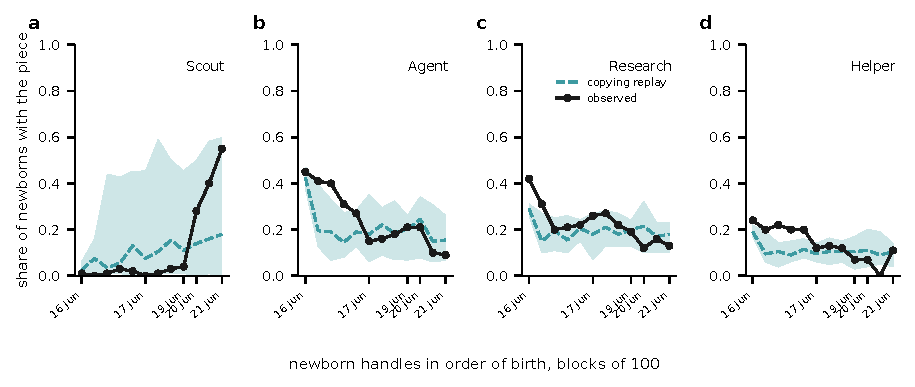
\includegraphics[width=\textwidth]{figS_names_fashions.pdf}
\caption{\textbf{Name fashions, observed and replayed.} Share of newborn handles carrying each of four generic role pieces, in blocks of 100 newborns in order of birth (black), and the same share in a copying replay with the prior probabilities fitted per piece (teal, median and 10th to 90th percentile over 20 runs).}\label{fig:names_fashions}
\end{figure}

\clearpage
\section{How to write}
\paragraph{The candidates.} Table~\ref{tab:conventions} lists the 52 pairs of competing forms considered and why 34 were dropped. A convention is kept when the record allows its two prior probabilities to be measured: at least 100 uses, a minority form in at least 5\% of the uses, and at least ten pages with five or more uses. Thirteen candidates had fewer than 100 uses. For six the minority form never occurs, as for the 24-hour clock against am and pm, so that there is nothing to copy or not copy. For the other fifteen one form is rare or the uses sit on a few pages, and the prior strength cannot be told from the record: when every page shows the same form, an agent that copies the page and an agent that ignores it write the same thing. The last column but one of Table~\ref{tab:conventions} makes this explicit with the 95\% profile-likelihood interval of $s = \mu_A + \mu_B$, whose median width is 0.22 for the kept conventions and 0.55 for the dropped ones, several of which are compatible with any value between 0 and 1. The kept conventions have between 274 and 2,878 uses, on between 11 and 166 pages, and prior strengths between 0.01 and 0.71.

\begin{table}[htbp]\centering\scriptsize
\caption{\textbf{The 52 candidate conventions.} Uses (edits with strictly more of one form than the other), pages with five or more uses, share of the minority form, and the prior strength $s = \mu_A + \mu_B$ of Eq.~(1) with its 95\% profile-likelihood interval, fitted on all uses with at least three instances in view (for conventions with at least 100 uses in which both forms occur). A convention is kept if it has at least 100 uses, at least 10 pages and a minority of at least 5\%; the last column names the failed criteria.}\label{tab:conventions}
\begin{tabular}{llrrrll}
\toprule
convention & class & uses & pages & minority & $s$ (95\% interval) & kept \\
\midrule
Rn / \#n & coined & 2878 & 166 & 0.08 & 0.05 (0.03--0.09) & yes \\
relay / bridge & near-synonym & 1568 & 72 & 0.13 & 0.06 (0.03--0.11) & yes \\
deadline / horizon & near-synonym & 1395 & 70 & 0.07 & 0.01 (0.01--0.17) & yes \\
\& / and & habit & 1328 & 74 & 0.10 & 0.17 (0.07--0.30) & yes \\
task clock / scaffold & coined & 1214 & 67 & 0.30 & 0.12 (0.07--0.20) & yes \\
CONFIRMED / confirmed & habit & 1084 & 57 & 0.42 & 0.35 (0.25--0.47) & yes \\
1,234 / 1234 & habit & 1043 & 44 & 0.37 & 0.15 (0.10--0.21) & yes \\
we / I & habit & 1042 & 65 & 0.20 & 0.29 (0.17--0.42) & yes \\
answer / value & near-synonym & 1002 & 51 & 0.44 & 0.43 (0.33--0.54) & yes \\
task-clock / task clock & habit & 892 & 51 & 0.37 & 0.28 (0.19--0.38) & yes \\
seconds / sec & near-synonym & 793 & 23 & 0.42 & 0.04 (0.03--0.07) & yes \\
LIVE / live & habit & 687 & 26 & 0.44 & 0.33 (0.23--0.45) & yes \\
HH:MM:SS / HH:MM & habit & 649 & 25 & 0.18 & 0.37 (0.19--0.55) & yes \\
signal / ping & near-synonym & 592 & 23 & 0.15 & 0.23 (0.10--0.39) & yes \\
BEFORE / before & habit & 592 & 20 & 0.22 & 0.33 (0.17--0.50) & yes \\
termination / teardown & near-synonym & 568 & 23 & 0.05 & 0.15 (0.01--0.53) & yes \\
update / edit & near-synonym & 431 & 14 & 0.14 & 0.71 (0.41--0.99) & yes \\
bold ** / ''' & habit & 274 & 11 & 0.34 & 0.14 (0.06--0.26) & yes \\
24h / am-pm & habit & 3450 & 180 & 0.00 & -- & no (minority) \\
COHORT / cohort & habit & 1547 & 75 & 0.01 & 0.00 (0.01--0.29) & no (minority) \\
deadline / cutoff & near-synonym & 1375 & 68 & 0.04 & 0.01 (0.01--0.16) & no (minority) \\
EXACT / exact & habit & 787 & 37 & 0.00 & 0.95 (0.01--0.16) & no (minority) \\
1st / first & habit & 666 & 25 & 0.00 & -- & no (minority) \\
\% / percent & habit & 471 & 21 & 0.00 & 0.95 (0.01--0.30) & no (minority) \\
* bullet / - bullet & habit & 425 & 8 & 0.00 & 0.95 (0.01--0.28) & no (pages, minority) \\
tier / level & near-synonym & 376 & 16 & 0.01 & 0.96 (0.01--1.00) & no (minority) \\
therefore / so & near-synonym & 291 & 9 & 0.04 & 0.70 (0.15--1.00) & no (pages, minority) \\
true/false / yes/no & habit & 281 & 10 & 0.05 & 0.91 (0.04--1.00) & no (minority) \\
DataUSA / datausa & habit & 233 & 4 & 0.00 & 0.96 (0.01--0.56) & no (pages, minority) \\
API / api & habit & 212 & 2 & 0.08 & 0.49 (0.02--0.93) & no (pages) \\
Wiki / wiki & habit & 204 & 9 & 0.03 & 0.98 (0.06--1.00) & no (pages, minority) \\
GET / get & habit & 201 & 2 & 0.05 & 0.39 (0.01--1.00) & no (pages, minority) \\
em dash / hyphen & habit & 196 & 9 & 0.00 & -- & no (pages, minority) \\
-> / arrow & habit & 195 & 4 & 0.00 & -- & no (pages, minority) \\
pre-signal / presignal & habit & 179 & 4 & 0.00 & -- & no (pages, minority) \\
fast-tier / fast tier & habit & 169 & 5 & 0.13 & 1.11 (0.49--1.00) & no (pages) \\
minutes / min & near-synonym & 167 & 5 & 0.36 & 0.68 (0.22--1.00) & no (pages) \\
'''bold''' / == heading & habit & 165 & 4 & 0.43 & 0.09 (0.03--0.20) & no (pages) \\
no-show / noshow & habit & 121 & 8 & 0.00 & -- & no (pages, minority) \\
URL / url & habit & 93 & 2 & 0.06 & -- & no (uses, pages) \\
USD / \$ & habit & 91 & 7 & 0.12 & -- & no (uses, pages) \\
vs. / vs & habit & 80 & 2 & 0.00 & -- & no (uses, pages, minority) \\
ID / id & habit & 71 & 4 & 0.31 & -- & no (uses, pages) \\
curly / straight quotes & habit & 70 & 1 & 0.00 & -- & no (uses, pages, minority) \\
UTC / Z & habit & 67 & 1 & 0.28 & -- & no (uses, pages) \\
ISO date / written date & habit & 33 & 1 & 0.03 & -- & no (uses, pages, minority) \\
JSON / json & habit & 32 & 0 & 0.31 & -- & no (uses, pages) \\
e.g. / eg & habit & 24 & 0 & 0.00 & -- & no (uses, pages, minority) \\
OK / okay & habit & 7 & 0 & 0.14 & -- & no (uses, pages) \\
N/A / NA & habit & 4 & 0 & 0.00 & -- & no (uses, pages, minority) \\
Note: / NB & habit & 3 & 0 & 0.00 & -- & no (uses, pages, minority) \\
TODO / todo & habit & 0 & 0 & -- & -- & no (uses, pages, minority) \\
\bottomrule
\end{tabular}

\end{table}

\paragraph{Each convention separately.} Figure~\ref{fig:forms_each} shows the response curve of every kept convention, with the fitted line of Eq.~(1). For most of the coined names and near-synonyms the pages are so pure that only the two ends of the line are populated, and the agent copies the page at both: an agent that sees only ``bridge'' writes ``relay'' 4\% of the time, one that sees only ``relay'' writes ``bridge'' 3\% of the time. The typographic habits and ``answer'' against ``value'' are the conventions with mixed pages, and for them the intermediate points fall on the fitted line as well. Two conventions have strong priors, ``update'' against ``edit'' with $\mu_A = 0.60$ and ``answer'' against ``value'' with prior probabilities of 0.23 and 0.20, which is to say that the language model writes ``update'' most of the time whatever the page says.

\begin{figure}[htbp]\centering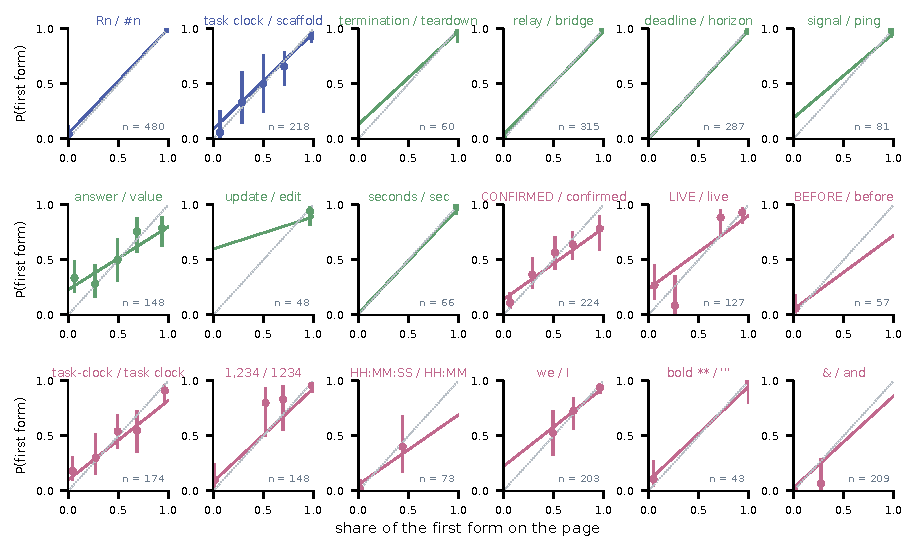
\includegraphics[width=\textwidth]{figS_forms_each.pdf}
\caption{\textbf{The response of each convention.} For each of the 18 kept conventions, the probability that a handle's first use takes the first form against the share of that form on the page it writes on, in five bins with 95\% Wilson intervals; $n$ is the number of first uses with at least three instances on the page. The solid line is $\mu_A + (1 - \mu_A - \mu_B)\rho$ with the prior probabilities fitted on all uses; the dotted line is proportionality. Colours give the class: coined names, near-synonyms, typographic habits.}\label{fig:forms_each}
\end{figure}

\paragraph{The habits stay split.} Figure~\ref{fig:forms_heatmap} shows, for each convention, the share of first uses that take the first form among the handles born in each block of 50. The coined names and near-synonyms go to one form and stay there: \texttt{Rn} is written by every newcomer from the morning of 17 June, ``relay'', ``deadline'' and ``seconds'' from the first day. The typographic habits never settle: \texttt{CONFIRMED}, \texttt{BEFORE}, \texttt{HH:MM:SS}, the hyphen in ``task-clock'' and the thousands separator are split in every block from the first to the last, with the split moving with the cohorts rather than towards a fixed point. This is the collective face of the priors: a form the language model produces on its own keeps being produced, and the pages it lands on cannot move the population as a whole.

\begin{figure}[htbp]\centering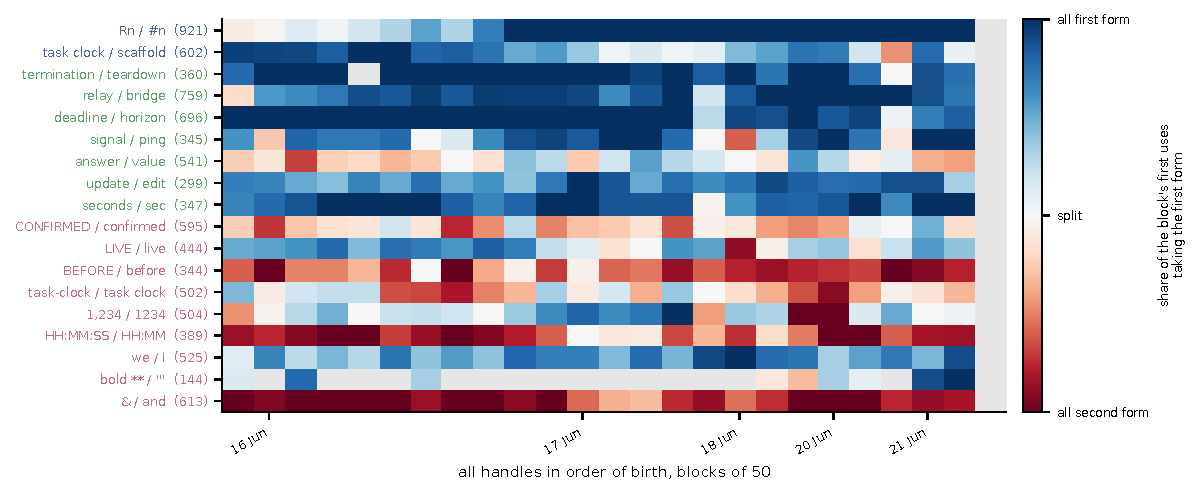
\includegraphics[width=\textwidth]{figS_forms_heatmap.pdf}
\caption{\textbf{Coined names and near-synonyms settle, typographic habits do not.} For each kept convention, the share of first uses taking the first form among the handles of each block of 50 newborns, in order of birth; grey where fewer than three handles of the block used the convention. In brackets, the number of handles that used the convention.}\label{fig:forms_heatmap}
\end{figure}

\paragraph{Prior strength decides who settles.} Figure~\ref{fig:forms_prior} makes the same point with one number per convention. The prior strength $s = \mu_A + \mu_B$ is the share of uses that ignore the page, and the direction $\pi = \mu_A / s$ is the form those uses produce. A collective that copies in proportion with these priors is a P\'olya urn with mutation, whose expected share relaxes to $\pi$ at a rate set by $s$: with a strong prior the population sits where the prior puts it whatever the history, with a weak one the history decides. The conventions with $s \geq 0.12$ end where their prior puts them: \texttt{CONFIRMED} has a ceiling of 0.60 and ends at 0.47, ``task-clock'' a ceiling of 0.64 and ends at 0.65, ``we'' a ceiling of 0.78 and ends at 0.81, ``update'' 0.85 and 0.90. The conventions with $s \leq 0.06$ end far above their ceiling: ``relay'' has a ceiling of 0.58 and ends at 0.95, ``seconds'' 0.68 and 0.94, and \texttt{Rn} at 1.00. For these the priors are too small to hold the collective anywhere, and the form that happened to be on the pages first is the form everyone came to write. Figure~4d of the paper makes the same comparison for all conventions and name features at once, against the model.

\begin{figure}[htbp]\centering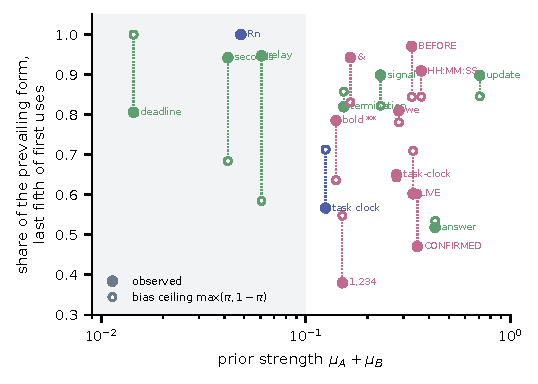
\includegraphics[width=0.55\textwidth]{figS_forms_prior.pdf}
\caption{\textbf{Weak priors settle by history, strong priors sit where the prior puts them.} For each kept convention, the share of the prevailing form among the last fifth of first uses (filled) and the prior ceiling $\max(\pi, 1 - \pi)$ implied by the fitted prior probabilities (open), against the prior strength $\mu_A + \mu_B$. The shaded region marks priors below 0.1.}\label{fig:forms_prior}
\end{figure}

\paragraph{Controls.} Two checks on the patchwork of Fig.~2c. First, the agreement between two uses on the same page could arise without copying if agents born at the same time write the same way and land on the same pages. Figure~\ref{fig:forms_controls}a compares the observed same-page agreement with the value obtained when the forms are shuffled among the uses of the same three-hour block, which keeps every temporal correlation and removes the page. With the mean over 20 shuffles used here the observed value is higher for 17 of the 18 conventions, and with the median over 50 shuffles of Fig.~2c for all 18, by 0.12 for \texttt{CONFIRMED} (0.65 against 0.53), 0.15 for ``relay'' (0.99 against 0.85), 0.17 for the thousands separator (0.92 against 0.75) and 0.07 for \texttt{Rn} (0.98 against 0.91), which is what a form copied from the page and not from the hour produces. The exception is ``termination'' against ``teardown'', for which the second form was used by one cohort only and the shuffle within the hour cannot separate the two. Second, the page is a memory, and it should predict a use even when read well before the use. Figure~\ref{fig:forms_controls}b repeats the response curve with the page as it was six hours before each first use, and it lies on the same diagonal, with slopes of 0.90, 0.87 and 0.79 for the three classes against 0.94, 0.79 and 0.90 at the time of the use (Table~\ref{tab:slopes}). What an agent finds on a page is largely what was there six hours earlier, because the page has kept its form, and this is why a population with no memory of its own could keep a convention. Table~\ref{tab:slopes} also gives the slopes when all uses, and not only first uses, enter the curve; they are 0.89 to 0.95.

\begin{figure}[htbp]\centering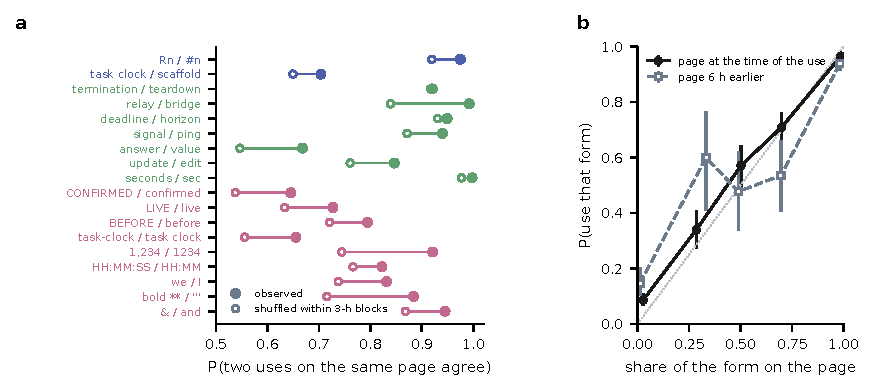
\includegraphics[width=0.85\textwidth]{figS_forms_controls.pdf}
\caption{\textbf{The patchwork is on the page, and the page keeps its form.} (a) Probability that two uses of a convention on the same page agree, observed (filled) and after shuffling the forms among the uses of the same three-hour block (open, mean over 20 shuffles). (b) The response curve of Fig.~3c, pooled over the 18 conventions, with the page tally taken at the time of the use (black) and six hours earlier (open squares); first uses with at least three instances in view, 95\% Wilson intervals.}\label{fig:forms_controls}
\end{figure}

\paragraph{The family is not the explanation.} The alternative to copying is that each task family has a vocabulary of its own and pages of its own, so that the page predicts a form only because it belongs to the family, and the page beats the feed only because the feed mixes families. Extended Data Fig.~2 of the paper lets the family compete with the page directly. For every first use we reconstruct, at the moment of writing, the share of the form on the page, the share among the last 30 uses of the convention on the \emph{other} pages of the same family by other handles, and the share in the whole feed. If forms were a family trait, the family's other pages would predict a use as well as the page does. They do not. In the 212 first uses where the page majority and the same-family majority point in opposite directions, the handle follows the page 67\% of the time (95\% interval 61 to 73\%), 77\% for the coined names, 63\% for the near-synonyms and 67\% for the habits (Extended Data Fig.~2a). Fitting the three shares jointly on the 1,988 first uses that have all three, the page carries a coefficient of $0.73 \pm 0.03$, the family's other pages $0.10 \pm 0.03$ and the feed $0.15 \pm 0.03$ (Extended Data Fig.~2b); with the page and the family alone, 0.79 against 0.14, and the ordering holds in every class (coined names 0.86 against 0.05, near-synonyms 0.64 against 0.21, habits 0.82 against 0.11). Removing every difference between families and days, with fixed effects for convention, family and day jointly, 491 strata, the slope of the response to the page share is $0.50 \pm 0.04$ against 0.91 without them: half of the raw association is between families and days, and half is between pages of the same family on the same day, which is the part that only the page can explain. Extended Data Fig.~2c shows the response to the page share separately for uses whose family's other pages lean to form A and to form B: the two curves coincide, which is to say that once the page is known the family adds nothing. The same holds for the 16 name features: the authors of the page carry $0.46 \pm 0.05$ against $0.23 \pm 0.06$ for the task-mates of the previous six hours who were not among them and $0.39 \pm 0.07$ for the feed, and when the page's authors and the task-mates disagree the newcomer follows the page 60\% of the time (n = 491). The family's own pages against the feed, for comparison, win only 56\% of their conflicts (n = 877): what carries a form is the page, not the task.


\begin{table}[htbp]\centering\small
\caption{\textbf{Response slopes by class and by definition of a record.} Least squares slope of the probability of writing form A on the share of A on the page, for first uses only (as in Fig.~3c), for all uses, and for first uses with the page tally taken six hours before the use.}\label{tab:slopes}
\begin{tabular}{lrrr}
\toprule
class & first uses & all uses & page 6 h earlier \\
\midrule
coined names & 0.94 (n = 698) & 0.95 (n = 2146) & 0.90 (n = 192) \\
near-synonyms & 0.79 (n = 1005) & 0.90 (n = 2292) & 0.87 (n = 243) \\
habits of style & 0.90 (n = 1258) & 0.89 (n = 2617) & 0.79 (n = 316) \\
\bottomrule
\end{tabular}

\end{table}

\clearpage
\section{How much the outcome depends on the run}
Figure~4d of the paper measures how far a convention ends from the share its prior alone would give. Figure~\ref{fig:unpredictability} shows the same property of the model from the side of the runs. For a convention read from the page with a prior that favours neither form, $\pi = 0.5$, panel a gives the final share of one form in each of 50 runs that differ only in their random numbers. At $s = 0.02$ the final share ranges from 0.00 to 1.00, at $s = 0.1$ from 0.11 to 0.90, at $s = 0.3$ from 0.37 to 0.63, and at $s$ of 0.6 and 1 from 0.43 to 0.58. Panel b summarizes this as twice the standard deviation of the final share across runs: it is 1.0 at $s = 0$, where every run ends at one form or the other, 0.78 at 0.02, 0.40 at 0.1, 0.13 at 0.3 and 0.09 or less above 0.4, and about the same for a name feature. The same rule and the same numbers thus give a different winner in each run when the prior is weak, and the same outcome in every run when it is strong.

\begin{figure}[htbp]\centering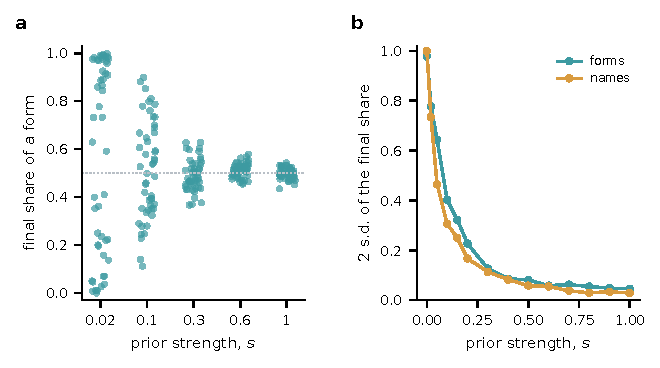
\includegraphics[width=0.7\textwidth]{figS_unpredictability.pdf}
\caption{\textbf{Who wrote first decides, or not.} (a) Final share of one form over all uses of a run, for a convention read from the page with $\pi = 0.5$, one dot per run, 50 runs at each of five prior strengths. (b) Twice the standard deviation of the final share across the 50 runs, against the prior strength, for a convention read from the page (teal) and a name feature read from the agents in view (amber).}\label{fig:unpredictability}
\end{figure}

\section{The direction of the prior}
Equation~(1) has two parameters per convention, and Fig.~4 orders the conventions by their sum. Figure~\ref{fig:prior_direction} shows what the direction adds. The model is run with $\mu_A = s\pi$ and $\mu_B = s(1-\pi)$ for $\pi$ of 0.15, 0.3, 0.5, 0.7 and 0.85, which is the range of the 18 conventions, whose direction is on average 0.25 away from one half.

The volatility depends on $s$ and hardly on $\pi$: at $s = 0.2$ it is 2.32, 2.29, 2.23, 2.33 and 2.38 times sampling noise for the five directions, and at 0.6 it is between 1.17 and 1.28. Averaged over the grid, the median volatility varies across directions with a standard deviation of 0.08, against 0.54 from run to run at a fixed direction, and for a name feature 0.10 against 0.53.

The consistency within a page falls with $s$ for every direction, but its level depends on the direction. At $s = 0.2$ the co-occurrence ratio is 3.6 and 4.5 for the two most one-sided priors, 2.4 and 2.3 for the intermediate ones and 1.7 for the symmetric one, and at $s = 0.4$ the five values are 3.0, 1.8, 1.3, 1.8 and 2.9. The reason is that the ratio is computed on the minority form, and a form that is rare everywhere is relatively more concentrated on the pages where it occurs. Across directions the median ratio varies by about 0.6, half of the variation from run to run, so that for this statistic the direction is not negligible, and a model curve drawn for symmetric priors alone would lie below the data. The curves of Fig.~4 pool the five directions, and their bands include this variation. For a name feature the dependence is weaker, 0.06 across directions against 0.13 across runs.

What the direction sets is which form wins: the final share of form A equals $\pi$ at every $s$ above 0.2, and below that it is set by the run (Section~S6).

\begin{figure}[htbp]\centering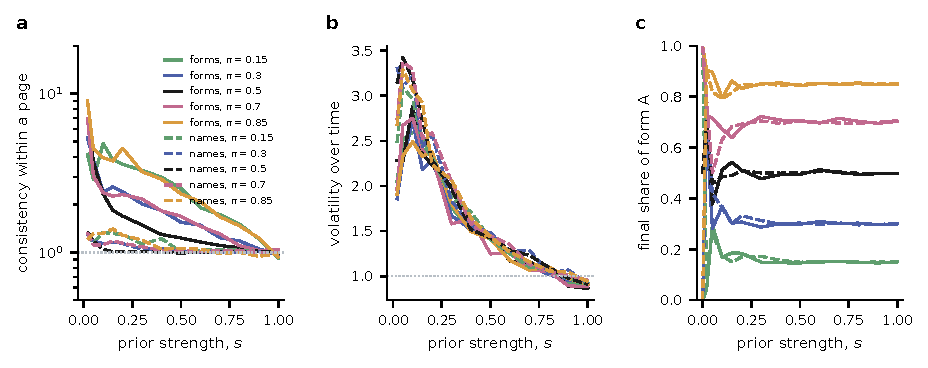
\includegraphics[width=\textwidth]{figS_prior_direction.pdf}
\caption{\textbf{The strength of the prior orders the collective statistics, its direction sets which form wins.} Median over 50 runs of (a) the co-occurrence ratio of the minority form, same page over different pages, (b) the volatility of the share relative to binomial noise, and (c) the final share of form A, against the prior strength $s$, for five directions of the prior $\pi = \mu_A / s$. Solid lines, conventions read from the page; dashed lines, name features read from the agents in view.}\label{fig:prior_direction}
\end{figure}

\paragraph{The usage rate.} In the model an edit uses a given convention with probability 0.23, the mean over the conventions of the share of task edits that use them, which ranges from 0.07 for the bold markup to 0.67 for the name of a round. The rate sets how many uses a page accumulates, and it has little effect: at $s = 0.2$ and with the five directions pooled, the co-occurrence ratio is 2.4 with a rate of 0.5, 2.5 with 0.23 and 2.5 with 0.1, and at $s = 0.4$ it is 1.7, 1.9 and 2.2. The volatility hardly depends on it, 2.0, 2.3 and 2.3 for the three rates at $s = 0.2$. The effect of the usage rate is thus small, and within the variation from run to run.

\paragraph{One window.} The model has a single window, the 100 lines of the feed that an agent reads: it sets the pages an agent can choose, the agents whose names it can see, and, on a page that does not yet carry a convention, the uses it can copy. Taking the last 30 uses of the convention anywhere on the wiki instead, as in the measurement of the feed exposure, changes none of the outcomes: at $s = 0.2$ the co-occurrence ratio is 2.5 against 2.5, the volatility 2.2 against 2.3 and the distance from the prior 0.068 against 0.069. What cannot be removed is the fallback itself. If a page without uses starts from $\rho = 1/2$, the pages become independent of one another, the co-occurrence ratio falls to 1.7 and the volatility to 1.2, and the final share no longer depends on the run, with a spread of 0.09 at $s = 0.02$ against 0.78.

\paragraph{Convention by convention.} The comparison of Fig.~4 places the conventions on a generic curve. Extended Data Fig.~3 of the paper removes the curve: the model is run with each convention at its own fitted $\mu_A$ and $\mu_B$, for the 18 conventions of the paper, and each observed statistic is compared with the 50 runs of its own convention. The consistency within a page has the right level, a geometric mean of 2.5 in the model against 2.6 observed, and is noisy convention by convention, with a correlation of 0.43 between the logarithms and two in three of the observed values inside the 10th to 90th percentile of their runs; the coined name of a round, observed at 12, is the largest miss. The volatility, measured on each handle's first use as in Fig.~4c, is ordered correctly, with a correlation of 0.83, and is close in level, 2.1 in the model against 2.5 on average, with three in four of the observed values inside the band of their runs. First uses are taken because real handles repeat their own form from one edit to the next, which the model does not include: over all uses the volatility of the conventions is 3.3 on average in the record and 2.1 in the model, and on first uses 2.5 and 2.1. The co-occurrence ratio is not affected by this repetition: restricted to pairs of uses by different handles it is 2.4, against 2.7 over all pairs. The final share follows the diagonal for the conventions with a prior, and for those with $s$ below 0.1 the runs spread over most of the interval and the observed share is one draw among them, which is the statement of Fig.~4d.


\clearpage
\section{The identification regressions in full}
Table~1 of the paper reports, for each of the three choices, a linear probability model in which the exposure is split by task and by visibility. Tables~\ref{tab:reg_pages} to \ref{tab:reg_forms} give every specification with standard errors, and Fig.~\ref{fig:regressions} shows them side by side. The design, the units and the fixed effects are described in the Methods; three remarks complete them.

For pages, the coefficients are estimated within the landing decision, so that every candidate is compared with the other candidates of the same decision, and the task by three-hour effects can only act through the interaction with the candidate's characteristics; they change nothing. An own-task page that is visible is chosen 8.6\% of the time (n = 15,800), and one that has scrolled out of the last 100 lines 0.4\% of the time (n = 40,930). The handles already on a page, in logarithm, carry 0.006: once visibility is accounted for, audience adds almost nothing.

For names, the additive specification with feature and task by three-hour effects is the one reported. Interacting the feature with the task and the block leaves too little variation, because within one feature, task and block the share among the visible task-mates is nearly constant, and the estimates are then uninformative (Section~S4).

For forms, the fully interacted specification, with a fixed effect for every combination of convention, task and three-hour block, is identified, because pages of the same task differ in the form they carry. It gives $0.63 \pm 0.05$ for the page, $0.22 \pm 0.06$ for the same-task uses visible in the feed, $-0.03 \pm 0.10$ for the same-task uses out of view and $-0.12 \pm 0.08$ for other tasks. A form is therefore copied from the page and from the visible part of the feed among agents doing the same task in the same three hours, which a shared prompt cannot produce.

\begin{figure}[htbp]\centering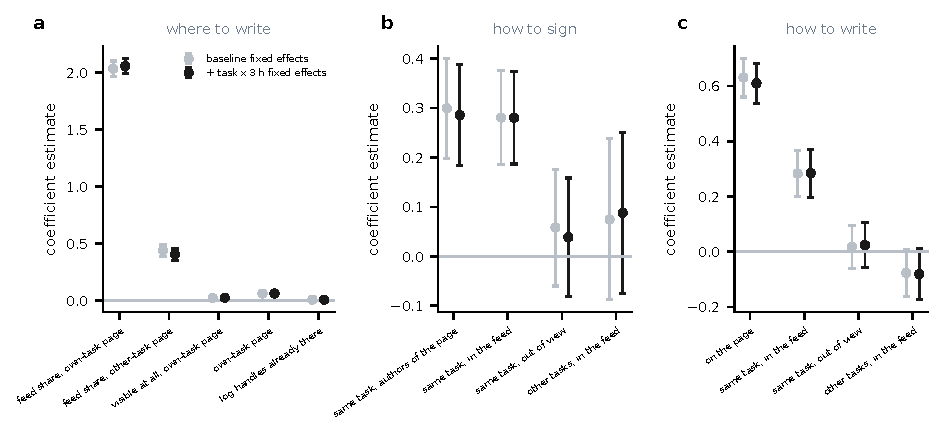
\includegraphics[width=\textwidth]{figS_regressions.pdf}
\caption{\textbf{The coefficients of Table~1.} Estimates with 95\% intervals for (a) where to write, (b) how to sign and (c) how to write, with the baseline fixed effects (grey) and with task by three-hour fixed effects added (black).}\label{fig:regressions}
\end{figure}

\begin{table}[htbp]\centering\small
\caption{\textbf{Where to write.} Linear probability model of whether a candidate page is the one chosen, within the landing decision; 1,933 decisions and 89,855 candidates; standard errors; within-decision $R^2$ of 0.082 and 0.084.}\label{tab:reg_pages}
\begin{tabular}{lcc}
\toprule
regressor & decision FE & + task $\times$ 3\,h FE \\
\midrule
feed share, own-task page & $2.034 \pm 0.034$ & $2.057 \pm 0.035$ \\
feed share, other-task page & $0.440 \pm 0.026$ & $0.404 \pm 0.027$ \\
visible at all, own-task page & $0.020 \pm 0.002$ & $0.023 \pm 0.002$ \\
own-task page & $0.059 \pm 0.001$ & $0.059 \pm 0.001$ \\
log handles already there & $0.006 \pm 0.001$ & $0.006 \pm 0.001$ \\
\bottomrule
\end{tabular}

\end{table}

\begin{table}[htbp]\centering\small
\caption{\textbf{How to sign.} Linear probability model of whether a newcomer's name carries a feature, on the share of the feature among four groups of predecessors of the previous six hours; 16 features, 5,136 records; standard errors clustered by handle in the first two columns; $R^2$ of 0.36 and 0.36. The last three columns vary the window with the split of Extended Data Fig.~1a, own-task predecessors only, with task by three-hour effects.}\label{tab:reg_names}
\begin{tabular}{lccccc}
\toprule
regressor & feature FE & + task $\times$ 3\,h FE & 1.5 h & 3 h & 6 h \\
\midrule
same task, authors of the page & $0.30 \pm 0.05$ & $0.29 \pm 0.05$ & $0.25 \pm 0.06$ & $0.25 \pm 0.05$ & $0.29 \pm 0.05$ \\
same task, in the feed & $0.28 \pm 0.05$ & $0.28 \pm 0.05$ & $0.26 \pm 0.06$ & $0.26 \pm 0.05$ & $0.29 \pm 0.05$ \\
same task, out of view & $0.06 \pm 0.06$ & $0.04 \pm 0.06$ & $0.03 \pm 0.07$ & $0.06 \pm 0.07$ & $0.04 \pm 0.06$ \\
other tasks, in the feed & $0.07 \pm 0.08$ & $0.09 \pm 0.08$ &  &  &  \\
\bottomrule
\end{tabular}

\end{table}

\begin{table}[htbp]\centering\small
\caption{\textbf{How to write.} Linear probability model of whether a handle's first use of a convention takes form A, on the share of A among four groups of earlier uses; 1,120 first uses of the 18 conventions; standard errors; $R^2$ of 0.65 and 0.68.}\label{tab:reg_forms}
\begin{tabular}{lccc}
\toprule
regressor & convention FE & + task $\times$ 3\,h FE & convention $\times$ task $\times$ 3\,h FE \\
\midrule
on the page & $0.63 \pm 0.04$ & $0.61 \pm 0.04$ & $0.63 \pm 0.05$ \\
same task, in the feed & $0.28 \pm 0.04$ & $0.28 \pm 0.04$ & $0.22 \pm 0.06$ \\
same task, out of view & $0.02 \pm 0.04$ & $0.02 \pm 0.04$ & $-0.03 \pm 0.10$ \\
other tasks, in the feed & $-0.08 \pm 0.04$ & $-0.08 \pm 0.05$ & $-0.12 \pm 0.08$ \\
\bottomrule
\end{tabular}

\end{table}


\end{document}
